% !TEX program = pdfLaTeX
\documentclass{scrartcl}
\usepackage[utf8]{inputenc}
\usepackage[T1]{fontenc} 
\usepackage[bitstream-charter]{mathdesign}
\usepackage{fetamont,url,tikz,verbatim,listings,inconsolata}
\usetikzlibrary{positioning}
\setkomafont{sectioning}{\rmfamily\bfseries\boldmath}
\renewcommand{\descriptionlabel}[1]{\hspace{\labelsep}\texttt{#1}}
\title{mf2outline}
\author{Linus Romer}

\lstset{basicstyle=\footnotesize\ttfamily,breaklines=true}

\begin{document}	
%
\maketitle
%
\tableofcontents
%
\section{Introduction}
%
\MF{} is a very versatile font description language, especially when you need to design several faces of a typeface family. However, the \MF{} compiler has some severe restrictions:
\begin{itemize}
	\item The \MF{} compiler can only produce bitmaps and cannot produce outline font formats like Type~1 or OpenType.
	\item The \MF{} compiler cannot write more than 256 different characters per font.
\end{itemize}
Luckily, the \MP{} language and its compiler can be used as an expediant (see \cite{hobby13}). Together with the \verb|mfplain.mp| base, the \MP{} language supersets nearly 100~\% of the \MF{} language. The \MP{} compiler outputs PostScript files, which can be imported in FontForge and then be converted to outline font formats. This process is automated by the \verb|mf2outline.py| script. 

For compatiblity reasons, the \verb|mfplain.mp| base does not support more than 256 different characters per font. To get over this and other artificial restriction, the \verb|mf2outline.mp| base extends the capabilities of the \verb|mfplain.mp| base. Of course, the backwards compatibility to \MF{} will be lost by using these extensions.

\begin{center}
	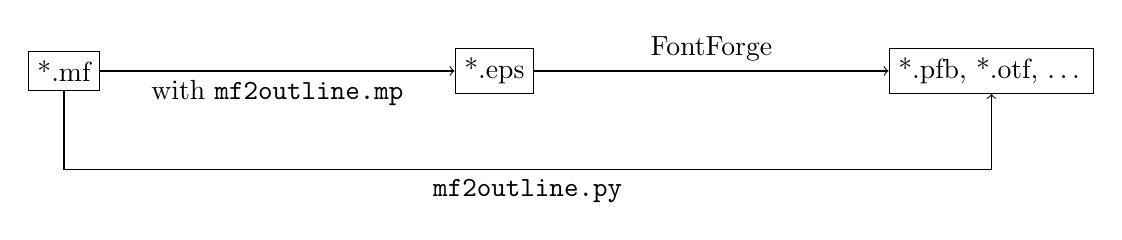
\begin{tikzpicture}[node distance=4.5cm]  
		\node[rectangle,draw](mf){*.mf};
		\node[rectangle,draw,right=of mf](eps){*.eps};
		\node[rectangle,draw,right=of eps](pfb){*.pfb, *.otf, \ldots};
		\draw[->] (mf.east) -- (eps.west) node[pos=.5,above]{\MP} node[pos=.5,below]{with \verb|mf2outline.mp|};
		\draw[->] (eps.east) -- (pfb.west) node[pos=.5,above]{FontForge};
		\draw[->] (mf.south) -- ++(0,-1) -| (pfb.south) node[pos=.25,below]{\verb|mf2outline.py|};
	\end{tikzpicture}
\end{center}
%
\section{The \texttt{mf2outline.py} Script}
%
\subsection{Requirements}
%
The following programs have to be installed before using \verb|mf2outline|:
%
\begin{itemize}
	\item Python interpreter (\verb|mf2outline.py| is a Python script)
	\item \MP{} compiler
	\item FontForge's python extension (\verb|python-fontforge|)
\end{itemize}
%
\subsection{Usage and Command-line Options}
%
The general usage for a \MF{} file \verb|mfsource| is easy:
\begin{verbatim}
	mf2outline.py mfsource
\end{verbatim}
%
This will output an OpenType font file named \verb|mfsource.otf| in your working directory. The file extension \verb|.mf| of the specified \MF{} source file can be omitted.

You may add some of these optional arguments:
\begin{description}
	\item[-h, -{}-help] \hfill \\
		Show the help message and exit.
	\item[-v, -{}-verbose ] \hfill \\
		Explain what is being done.
	\item[-vv, -{}-veryverbose] \hfill \\
		Explain very detailed what is being done.
	\item[-{}-designsize SIZE] \hfill \\
		Force the designsize to be SIZE (e.g. 12 for 12pt).
	\item[-{}-raw] \hfill \\
		Do not remove overlaps, round to int, add extrema, add hints\ldots
	\item[-{}-preview  ] \hfill \\
		Generate only the most important letters, use icosagon pens instead of circle/elliptic pens and do not care about advanced font features like kerning and ligatures (mainly used for \textffm{METAFLOP}).\\
		List of letters: ! \& ( ) , - . / 0 1 2 3 4 5 6 7 8 9 ? A B C D E F G H I J K L M N O P Q R S T U V W X Y Z a b c d e f g h i j k l m n o p q r s t u v w x y z 
	\item[-f FORMATS, -{}-formats FORMATS] \hfill \\
		Generate outline fonts in the formats FORMATS (comma separated list).\\
		Supported formats: sfd, afm, pfa, pfb, otf, ttf, eoff, svg, tfm\\
		Default: otf
	\item[-{}-encoding ENC ] \hfill \\
		Force the font encoding to be ENC.\\
		Natively supported encodings: ot1, t1, unicode\\
		Default: unicode\\
		The file ENC.enc will be read if it exists in the same directory as the source file (the encoding name inside the encoding file must be named ENC, too).
	\item[-{}-fullname FULL] \hfill \\
		Set the full name to FULL (with modifiers and possible spaces).
	\item[-{}-fontname NAME] \hfill \\
		Set the font name to NAME (with modifiers and without spaces).
	\item[-{}-familyname FAM] \hfill \\
		Set the font family name to FAM.
	\item[-{}-fullname-as-filename] \hfill \\
		Use the fullname for the name of the output file.
	\item[-{}-fontversion VERS] \hfill \\
		Set the version of the font to VERS.\\
		Default: 001.001
	\item[-{}-copyright COPY] \hfill \\
		Set the copyright notice of the font to COPY.
	\item[-{}-vendor VEND] \hfill \\
		Set the vendor name of the font to VEND (limited to 4 characters).
	\item[-{}-weight WGT] \hfill \\
		 Force the OS/2 weight of the font to be WGT.\\
		 The weight number is mapped to the following PostScript weight names:
		 \begin{itemize}
		 	\item[100] Thin
		 	\item[200] Extra-Light
		 	\item[300] Light
		 	\item[400] Book
		 	\item[500] Medium 
		 	\item[600] Demi-Bold
		 	\item[700] Bold
		 	\item[800] Heavy
		 	\item[900] Black
		 \end{itemize}
	\item[-{}-width WDT] \hfill \\
		Force the OS/2 width of the font to be WDT.\\
		 The width number stands for the following width names:
		 \begin{itemize}
		 	\item[1] Ultra-condensed
		 	\item[2] Extra-condensed
		 	\item[3] Condensed
		 	\item[4] Semi-condensed
		 	\item[5] Medium (normal)
		 	\item[6] Semi-expanded
		 	\item[7] Expanded
		 	\item[8] Extra-expanded
		 	\item[9] Ultra-expanded
		 \end{itemize}
	\item[ -{}-ffscript FFSCRIPT] \hfill \\
		Specify an own finetuning fontforge script (e.g. finetune.pe). The script file has to be in the same directory as the source file. Example script:\\
		\verb|Open($1);|\\
		\verb|SelectAll();|\\
		\verb|RemoveOverlap();|\\
		\verb|Generate($1);|\\
		\verb|Quit(0);|
\end{description}
%
\subsection{Restrictions}
%
Not every valid \MF{} typeface can be automatically converted by \verb|mf2outline|. The three most important restrictions are listed below:
\begin{itemize}
	\item The \MF{} typeface cannot be compiled by \MP{} when it uses some special features of \MF{} that are not implemented in \MP{} (e.g. \emph{Pandora}).
	\item If the font uses many overlapping filldrawn areas, FontForge does not always import the PostScript files correctly (e.g. Computer Modern). As a solution, you can use the \verb|--raw| option and finetune the font by hand in FontForge.
	\item As a mathematical fact, a generic cubic beziér spline path that is drawn by a elliptic pen cannot be converted perfectly to cubic beziér spline outlines. Hence, FontForge does only an approximation job here. This approximation is normally very close to the original shape, but if you use heavily twisted cubic beziér splines, the approximation will be unsatisfactory.
\end{itemize}
%
\subsection{\textffm{METAFLOP}}
%
\textffm{METAFLOP} is an easy to use web application for modulating \MF{} fonts:
\begin{center}
	\url{http://www.metaflop.com/modulator}
\end{center}
The conversion to outline formats is being done by \verb|mf2outline|. 
%
\subsection{Other Tools}
%
The following two programs are alternatives to \verb|mf2outline|.
%
\begin{description}
	\item[mftrace] is a python script that converts \MF{} fonts into Type~1 fonts. Unlike \verb|mf2outline|, \verb|mftrace| can cope with \emph{every} valid \MF{} font. Unfortunately, the outline paths are not that neat.
	\item[mf2pt1] is a perl script that converts \MF{} fonts into Type~1 fonts. Actually, \verb|mf2pt1| is pretty similar to \verb|mf2outline|, but does not rely that much on FontForge.
\end{description}
%
Both programs, \verb|mftrace| and \verb|mf2pt1|, have deeply inspired the author of \verb|mf2outline|. Thus, many ideas of the two programs can be found in \verb|mf2outline|, too.
%
\section{The \texttt{mf2outline.mp} Base}
%
The \texttt{mf2outline.mp} base extends the \texttt{mfplain.mp} base. Unlike \texttt{mf2outline.mp} base, \texttt{mf2outline.mp} causes \MP{} to write special additional glyph information to the PostScript files and to generate an additional file mf2outline.txt, that contains general font information. Normally, some of these additional information are stored in the \texttt{tfm} file.

There is a special version called \texttt{mf2outline-prev.mp} that causes \MP{} to use icosagon pens instead of circular/elliptic pens. The only difference to \texttt{mf2outline.mp} is the version number, that ends with the string \texttt{"prev"}.

Example of a \texttt{mf2outline.txt} file:
\begin{lstlisting}
mf2outline: font_size 10
mf2outline: font_slant 0
mf2outline: font_normal_space 2.29996
mf2outline: font_normal_shrink 0.80002
mf2outline: font_x_height 4.34998
mf2outline: font_quad 6.90002
mf2outline: font_os_weight 400
mf2outline: font_os_width 5
mf2outline: font_identifier FQDR
mf2outline: font_coding_scheme Unicode
mf2outline: font_copyright Linus Romer, 2015
mf2outline: font_name Quindesch-Regular10
mf2outline: font_fullname Quindesch Regular 10
mf2outline: font_familyname Quindesch
mf2outline: kerningclassesl 
0041 
0056 0057 
mf2outline: kerningclassesr 
0041 
0056 0057 
mf2outline: kerningmatrix 
0 -1.0994 
-1.0994 0 
mf2outline: gsubtable liga
0066 0066 
FB00 
mf2outline: gsubtable smcp
0068 
E02A 
mf2outline: gsubtable c2sc
0041 
E000 
0048 
E02A 
mf2outline: eof
\end{lstlisting}

Snippet from a PostScript file containing special \texttt{mf2outline} information:\lstset{language=PostScript} 
\begin{lstlisting}
% mf2outline: charwd 7.28752
% mf2outline: charht 6.49994
% mf2outline: chardp 0
% mf2outline: charic 0
% mf2outline: charcode 79
% mf2outline: charext 0
% mf2outline: charunicode 004F
\end{lstlisting}

The new extensions and its necessary macros are described in the following subsections.
%
\subsection{Additional Font and Glyph Parameters}
%
The \texttt{tfm} file stores amongst other things the following parameters:
\begin{itemize}
	\item Global font parameters:
	\begin{itemize}
		\item font\_size
		\item font\_slant
		\item font\_normal\_space
		\item font\_normal\_stretch
		\item font\_normal\_shrink
		\item font\_x\_height
		\item font\_quad
		\item font\_extra\_space
		\item font\_identifier (normally not stored)
		\item font\_coding\_scheme (normally not stored)
	\end{itemize}
	\item Glyph parameters:
	\begin{itemize}
		\item charwd (character width)
		\item charht (character height)
		\item chardp (character depth)
		\item charic (character italic correction)
		\item charcode (code number of the character)
		\item charext (code extension number of the character)
		\item chardx (horizontal escapement of glyph positioning)
		\item chardy (vertical escapement of glyph positioning)
	\end{itemize}
\end{itemize}
The \texttt{mf2outline.mp} base defines some new parameters that cannot be stored in the \texttt{tfm} format:
\begin{itemize}
	\item Global font parameters:
	\begin{itemize}
		\item font\_os\_weight
		\item font\_os\_width
		\item font\_version
		\item font\_copyright
		\item font\_name
		\item font\_fullname
		\item font\_familyname
	\end{itemize}
	\item Glyph parameters:
	\begin{itemize}
		\item charunicode (unicode string like "004A")
	\end{itemize}
\end{itemize}
%
\subsection{Unicode Support}
%

%
\subsection{Kerning}
%
\subsection{Ligatures}
%
\subsection{Other OpenType Features}
%

%
\begin{thebibliography}{Hobby13}
	\bibitem[Hobby13]{hobby13}
	John D. Hobby et al.
	\emph{\MP{} -- A User's Manual}.
	\url{www.tug.org/docs/metapost/mpman.pdf}, 2013
\end{thebibliography}
%
\end{document}
